\section{DECENTRALIZED EXPLORATION STRATEGY} 

At the core of our paper is a decentralized strategy for multi-robot exploration and mapping. The mobile robots exchange information about frontier points under the assumption of a fully connected graph and event based communication. If we define a mission as a process from getting a target point to reaching the same point, then all mobile robots communicate with each other in the moments when the mission for a single mobile robot is over. It means that the rest of mobile robots should send the data even though their missions are not over and they are still navigating to the goal. Event based communication is triggered by mission accomplishments.   

The exploration task is performed by a team of $n$ mobile robots  \(\text{$\mathcal {R}$}\) = $ \{ 1, 2,..., N\}$ where the mobile robots do not have prior knowledge about the environment, i.e., the position of the boundaries and obstacles.  
Every mobile robot $i$ gets the list of frontier points  \(\text{$\mathcal {Y}$}\) = $ \{ 1, 2,..., M\}$ from filter module (Fig. \ref{fig:exploration-strategy}) in the moments when any of the mobile robots reaches the target point (when the mission is over). $M$ is the number of frontier points represented as a tuple ($x$, $y$), corresponding to the position in meter from the map origin. 

We define the frontier point weight $W$ as a function of cost $C$, utility $U$ and frontier occupancy $F$. Cost function $C$: $R_{xy}$ \(\rightarrow \text{$\mathbb{R}^{+}$}\) is a mapping from $R_{xy}$ to a positive real number.  If $i$ is the index of the mobile robot, and $j$ is the index of the frontier point, then $C_{ij}$ describes the cost of $i$th robot to visit the $j$th frontier point. The cost can be a function of time, energy or, like in our case, the estimated distance travelled by mobile robot to reach the target frontier point. The estimated distance is approximated using Euclidean distance between the mobile robot position $\boldsymbol{p_{i}}$ and the frontier point position $\boldsymbol{y_{j}}$:

\begin{equation}\small
    C_{ij}=d(\boldsymbol{p_{i}}, \boldsymbol{y_{j}}) = \sqrt{(p_{ix}-y_{jx})^{2}+(p_{iy}-y_{jy})^{2}}.
    \label{cost}
\end{equation}

The utility function $U_{ij}$: $R_{xy}$ \(\rightarrow \text{$\mathbb{R}^{+}$}\) returns a positive real number, and uses the occupancy grid \(\text{$\mathcal {M}$}\) to find the value for the specific frontier point. The cells of \(\text{$\mathcal {M}$}\) may be marked as explored space, unexplored space or obstacle. The utility function is proportional to the number of the unexplored cells $c$ within a fixed distance from the frontier point $y_{j}$ in the previous defined radius $r$: 

\begin{equation}
    U_{y_{j}} = \lambda_{u}c,
\end{equation}

where $\lambda_{u}$ is a constant determined experimentally. When the function $U_{y_{j}}$ is taken into account, the mobile robot will prefer frontier points that are surrounded by more unexplored space even if they are a little bit further. 
It is assumed that the mobile robot will detect all unexplored cells around the assigned frontier point after reaching it. 

The most important component is the frontier occupancy function $F_{ij}$, the 2-dimensional Gaussian function with the position of the mean in a frontier point and with the standard deviation \boldsymbol{\sigma} = \begin{bmatrix}
           r_{f} \\
           r_{f} 
   \end{bmatrix}.
   
 If the frontier point $y_{j}$, for which the mobile robot $i$ is calculating the weight, is in the range of radius $r_{f}$ from the position of an another mobile robot assigned point (\boldsymbol{y_{a}}); the value of the frontier occupancy function is calculated by Gaussian function, and zero otherwise:

\begin{equation}\label{eq:frontier_funct}
 F_{ij}=
\begin{cases} 
       \lambda_{f} e^{-\Big[\frac{(y_{jx} - y_{ax})^2}{2\sigma_{x}^2} + \frac{(y_{jy} - y_{ay})^2}{2\sigma_{y}^2}\Big]} & \text{if $d(\boldsymbol{y_{j}}, \boldsymbol{y_{a}})< r_{f}$}, \\
      \quad \quad \quad \quad \quad 0 & \text{otherwise}
   \end{cases}
\end{equation}

where $\lambda_{f}$ is an experimentally determined constant. 
The example of the frontier point $y_j$, assigned point $y_a$ and Gaussian function values inside the radius $r_f$ are shown in Fig. \ref{fig:gauss}.
The function $F_{ij}$ is used to prevent assigning the frontier point to the mobile robot B if that point is close to a point that is already assigned to mobile robot A.

\begin{figure}[t!]
	\centering
	\fbox{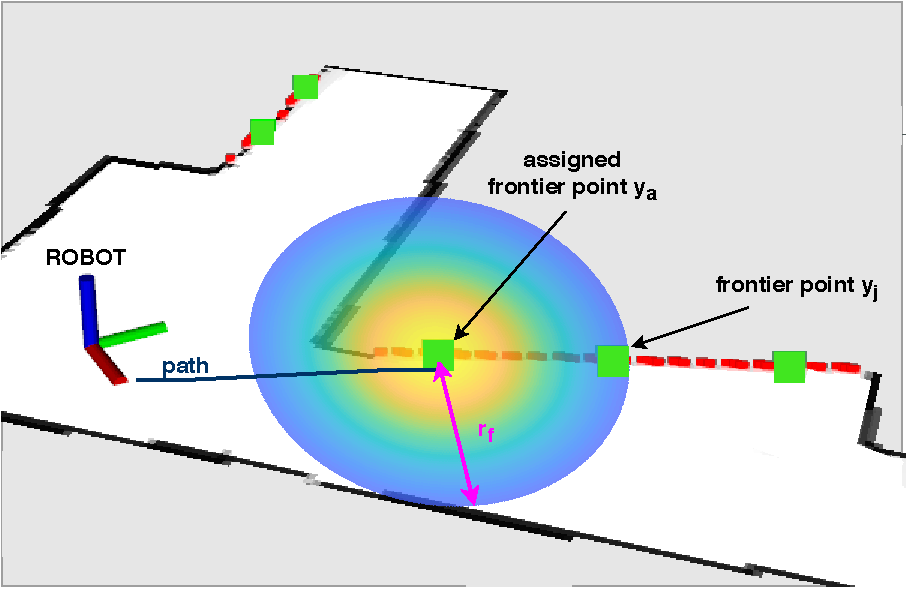
\includegraphics[width=0.95\columnwidth]{./Pictures/gauss.pdf}}
	\caption{A special scenario where the value of the frontier occupancy function $F$ is different from zero. Mobile robot is assigned to frontier point $y_a$, and follows the path to reach it. If another mobile robot calculates weight for the all current frontier points (green points), $F$ for frontier point $y_j$ is different from zero because $y_j$ is inside the radius $r_f$}.
	\label{fig:gauss}
\end{figure}

For each frontier point $y_{j}$, the weight $W_{ij}$ of the $i$-th mobile robot is calculated as: 
\begin{equation}
   {W}_{ij}= {C_{ij}} - {U_{y_{j}}} + {F_{ij}}.
   \label{weight}
\end{equation}

The weight matrix $\boldsymbol{W}$ ($N\times M$) is formed for $N$ mobile robots and $M$ frontier points: 

\begin{equation}
    \boldsymbol{W} = \begin{bmatrix}
    W_{00} & W_{01} & \hdots & W_{0j} & \hdots & W_{0M}\\
    W_{10} & \ddots & & & & \vdots\\
    \vdots & & \ddots & & &  \vdots \\
    W_{i0} & & & \ddots & & \vdots \\
    \vdots & & & & \ddots & \vdots\\
    W_{N0} & \hdots  & \hdots  & \hdots  & \hdots &    W_{NM}
    \end{bmatrix}.
\end{equation}

The mobile robots exchange information about their positions and current target points and make decisions for the future actions based on the exchanged information. The amount of exchanged data is thus reduced, which allows easier and faster communication.
The weight matrix $\boldsymbol{W}$ represents the input into the Hungarian algorithm that attempts to find an optimal assignment solution in polynomial time.

The Hungarian algorithm is described in \cite{Kuhn1955} and tested in \cite{Kulich2015}. Initially, the Hungarian algorithm assumes that the number of frontier points is the same as the number of mobile robots. Due to the fact that there are usually fewer mobile robots than frontier points, virtual mobile robots are added and then skipped during the process of assignment and exploration.

Let the matrix $X$ be the matrix of zeros and ones, where $X[i,j]=1$ iff the mobile robot $i$ is assigned to the frontier point $j$.
Than the optimal task assignment has weight:

\begin{equation}
     {\min_{X}}\ \Big(\sum_{i} \sum_{j} W_{ij}\ X_{ij}\Big),
\end{equation}

anticipating that minimisation of sum will ensure the dispersion of the mobile robots in the environment. 

\begin{algorithm}[t!]
\While{Unexplored}{
\If{Request}{
    Send position and current target point to the other mobile robots\;
    }
\If{Mobile robot $i$ has reached the previous target point}{
    Request positions and current target points from the other mobile robots\;
    \For{Each frontier point $y_{j}$}{
    Calculate the weight matrix $\boldsymbol{W}$\;
    Hungarian algorithm ($\boldsymbol{W}$)\;
    \textbf{return} Mobile robot $i$ is assigned to frontier point\;
    }
}
}
\label{algorithm1}
\caption{Decentralized strategy for mobile robot $i$}
\end{algorithm}


Our decentralized strategy executes during the robot motion and there are steps for each robot to be executed (\textbf{Algorithm 1}). All frontier points are visible to all mobile robots.
When mobile robot $i$ is assigned to frontier point according to line 10 in \textbf{Algorithm 1}, the mobile robot starts to follow the planned path and navigates to the target frontier point. Moreover, at the moment when the mobile robot $i$ reaches the target point (mission is over), a request is sent to the other mobile robots to get their positions and current target points, and to fill in the weight matrix $\boldsymbol{W}$, which is an input to Hungarian algorithm. The described process executes until the whole environment is explored, in other words, until a complete  map of the environment is generated. The Fig. \ref{fig:structure} illustrates the described steps and algorithm lines for a mobile robot team. 

\begin{figure}[h!]
    \centering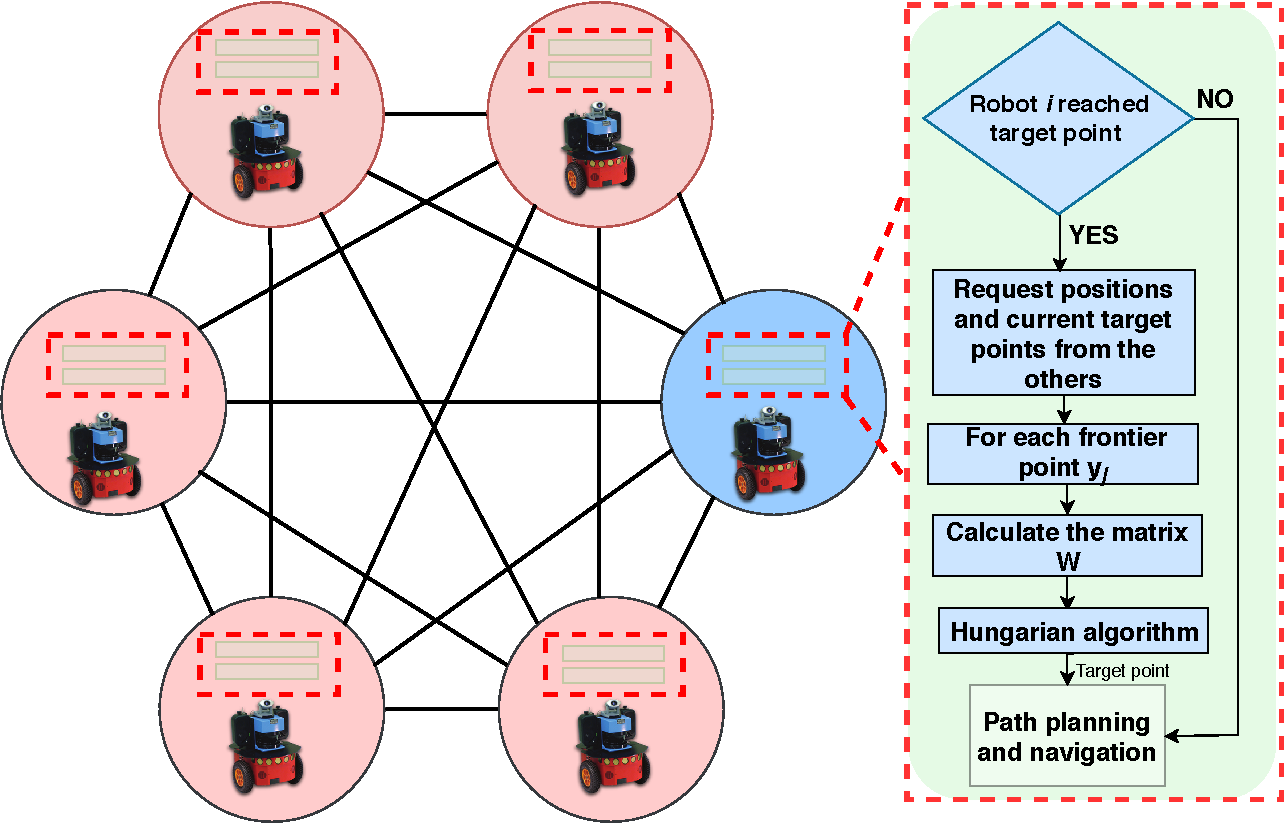
\includegraphics[width=1.0\columnwidth]{./Pictures/struktura_vol1.pdf}
	\caption{An execution of the decentralized part of the Fig. \ref{fig:exploration-strategy}. Every mobile robot explores the environment following the steps from \textbf{Algorithm 1}. The blue robot accomplished the mission and requests weights from the rest team memebers (red ones). The strategy is the same for all mobile robots and starts in the moment when each of them reaches the target point.}
   \label{fig:structure}
\end{figure}

